\documentclass[12pt]{article}
\usepackage[utf8]{inputenc}
\usepackage{amsmath, amssymb, url, float, graphicx, float}
\usepackage{algorithm, algpseudocode}
\usepackage[small,bf]{caption}
\usepackage{marginnote}
\usepackage[inner=1in, outer=2.5in, marginparsep=.5in, marginparwidth=1.5in]{geometry}

\usepackage{tikz}
\usetikzlibrary{arrows, positioning}

\newcommand{\norm}[1]{\left\|{#1}\right\|_2}
\newcommand{\tm}{\theta^\mathrm{max}}
\newcommand{\lagr}{\mathcal{L}}
\newcommand{\sinc}{\mathop{\mathrm{sinc}}}
\newcommand{\nnz}{\mathop{\bf nnz}}
\newcommand{\eps}{\varepsilon}
\newcommand{\complex}{\mathbf{C}}
\newcommand{\ii}{\mathbf{i}}
\newcommand{\id}{\mathbb{I}}
\newcommand{\efix}{e^\mathrm{fix}}
\newcommand{\ifix}{i^\mathrm{fix}}
\newcommand{\iinc}{i^\mathrm{inc}}
\newcommand{\tmax}{\theta^\mathrm{max}}
\newcommand{\tmin}{\theta^\mathrm{min}}
\newcommand{\gmax}{g^\mathrm{max}}
\newcommand{\gmin}{g^\mathrm{min}}
\newcommand{\smin}{s^\mathrm{min}}
\newcommand{\smax}{s^\mathrm{max}}
\newcommand{\kfix}{{k^\mathrm{fix}}}
\newcommand{\hp}{h^\mathrm{p}}
\newcommand{\qp}{q^\mathrm{p}}
\newcommand{\C}{\mathcal{C}}
\newcommand{\E}[1]{\mathbb{E}\left[#1\right]}
\newcommand{\lek}{\preceq}

\newcommand{\downto}{\downarrow}
\newcommand{\upto}{\uparrow}


\tikzstyle{box}=[draw, minimum size=1.5cm]
\tikzstyle{arr} = [thick,->,>=stealth]
\tikzstyle{arrb} = [thick, |--]

\renewcommand*{\marginfont}{\footnotesize}

\let\emptyset\varnothing

\input defs.tex

\bibliographystyle{alpha}

\title{Notes for HRP 204}
\date{Spring 2020}
\author{Guillermo Angeris}

\begin{document}

\maketitle

\section{Session 3 (April 14)}
The idea of this session is to add demography data in a (relatively) simple way
to the original SIR model.

\subsection{Definitions}

\paragraph{Survival curves.} The survival curve is a function which maps
the current age to its survival rate. (\ie, it takes in an age and outputs
the percentage of the population which survives to be greater than, or 
equal to this age. Another way of stating this is as the probability that
the age of death $X$ is greater than some given $\alpha$, $P(X \ge \alpha)$,
where $\alpha$ is the desired age.)

\paragraph{Mortality rate.} In the case that this curve follows an exponential
distribution, we will define the exponential parameter as the \emph{mortality
rate}, which we will write as $\mu \in \reals_+$.  This would then imply that
the area under the graph is the life expectancy, and would be equal to
$1/\mu$.\marginnote{This comes from the fact that $\E{X} = \int P(X \ge
x)\,dx$.} This also gives us a simple way of estimating the average mortality
rate for any given distribution by setting $\mu \approx 1/\E{X}$.

\subsection{Simple models}
The obvious `world's simplest model' is an easy one: let $S$ be the number of
susceptible individuals~\ref{fig:simplest-model} In this model, $S(t)$ is
always constant for all time (\ie, by definition $\dot S = 0$), and of course
has no interesting dynamics.

\begin{figure}[ht!]
\centering
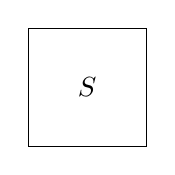
\begin{tikzpicture}
    \node [box](a) {$S$};
\end{tikzpicture}
\caption{World's simplest model.}
\label{fig:simplest-model}
\end{figure}

A slightly more complicated model (shown in
figure~\ref{fig:simple-model-deaths}) just includes the death rate as a `leaky
state.' In other words, the decay is given by $\dot S(t) = -\mu S(t)$, which has
the obvious solution
\[
    S(t) = S_0e^{-\mu t},
\]
a decaying exponential.

\begin{figure}[ht!]
\centering
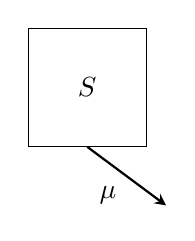
\begin{tikzpicture}
    \node [box](a) {$S$};
    \path (a.south) edge[arr] node[below left] {$\mu$} (1,-1.5);
\end{tikzpicture}
\caption{World's second simplest model.}
\label{fig:simple-model-deaths}
\end{figure}

Finally, an only slightly \emph{more} complicated model comes from adding
births (with rate $b \in \reals_+$) to the previous one (shown in
figure~\ref{fig:simple-model-births}). The result is the differential equation
$\dot S(t) = (b - \mu)S(t)$ with solution
\[
    S(t) = S_0e^{(b - \mu)t}.
\]
This is still an exponential (except when $b = \mu$, in which case the
population is constant).

\begin{figure}[ht!]
\centering
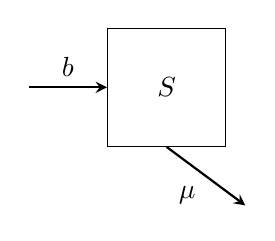
\begin{tikzpicture}
    \node [box](a) {$S$};
    \path (a.south) edge[arr] node[below left] {$\mu$} (1,-1.5);
    \path (-1.75, 0) edge[arr] node[above] {$b$} (a);
\end{tikzpicture}
\caption{World's third simplest model.}
\label{fig:simple-model-births}
\end{figure}

\subsubsection{Adding mortality in SIR}
Using the previous simple idea, we can then easily add death rates to the SIR
model.

\paragraph{Demography model.} A simple, basic assumption when adding birth
and death rates to the SIR model is to have the mortality rate be equal
for any of the three states, and, to prevent issues with normalization
we often assume that $\mu = b$.\marginnote{This ensures that the population is
always constant in  our model, so it can be normalized.} Note that this does
not include any excess mortality rates from the disease itself (we will deal
with this later). 


\begin{figure}[ht!]
\centering
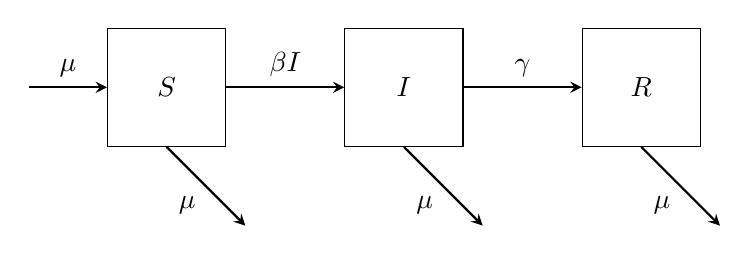
\begin{tikzpicture}[node distance=1.5cm, auto]
    \node [box](S) {$S$};
    \node [box, right=of S](I) {$I$};
    \node [box, right=of I](R) {$R$};

    \path (S.south) edge[arr] node[below left] {$\mu$} ++ (1,-1);
    \path (-1.75, 0) edge[arr] node[above] {$\mu$} (S);
    \path (I.south) edge[arr] node[below left] {$\mu$} ++ (1,-1);
    \path (R.south) edge[arr] node[below left] {$\mu$} ++ (1,-1);
    \path (S.east) edge[arr] node[above]{$\beta I$} (I);
    \path (I.east) edge[arr] node[above]{$\gamma$}(R);
\end{tikzpicture}
\caption{SIR incorporating deaths.}
\label{fig:sir-deaths}
\end{figure}

The new model equations (modeled in figure~\ref{fig:sir-deaths}) then are
\[
\begin{aligned}
    \dot S &= \mu - \beta IS - \mu S\\
    \dot I &= \beta IS - \gamma I - \mu I\\
    \dot R &= \gamma I  - \mu R.
\end{aligned}
\]

\paragraph{Simple properties.} We can give some simple thresholds and properties
of the system by analyzing interesting cases. For example, if infections are
`taking off,' then we must have
\[
    \dot I \ge 0 \implies \beta IS - \gamma I - \mu I \ge 0.
\]
Since $I \ge 0$ always, then we must have
\begin{equation}\label{eq:taking-off}
    \beta S - \gamma - \mu \ge 0 \implies S \ge \frac{\gamma + \mu}{\beta},
\end{equation}
\ie, that the susceptible proportion of the population must be greater than the
rate of recovery \emph{and} the rate of deaths and births divided by
$\beta$. We should note that this is larger than the SIR model without demographics since $\mu > 0$.\marginnote{Intuitively, this happens since we can view the total period of infectiousness as lasting roughly $1/(\gamma + \mu)$ rather than $1/\gamma$.}

With demography, we can then derive $R_0$ as the inverse of the susceptible
fraction
\[
    R_0 = \frac{\beta}{\gamma + \mu},
\]
which is always smaller than that of the non-demographic model.

\subsection{Equilibria}
We say a condition is at an \emph{equilibrium} if its relative proportions do not change
over time, \ie, if all time derivatives are zero. Additionally, we will say that
a disease is \emph{endemic} when it is at an equilibrium, but the infected
proportion is strictly positive.

\paragraph{Equilibria of SIR with demography.} To compute the equilibria,
we simply find $(S^*, I^*, R^*)$ such that
\[
    \dot S(t) = \dot I(t) = \dot R(t) = 0,
\]
simultaneously at these points. A rather simple and not terribly exciting
equilibrium is at $(S^*, I^*, R^*) = (1, 0, 0)$, \ie, no infections have
been introduced. We will call this the \emph{disease-free equilibrium}.

A second important equilibrium is the \emph{endemic equilibrium}, which happens
when, in the same way as~\eqref{eq:taking-off},
\[
    I^*(\beta S^* - \gamma - \mu) = 0,
\]
but, since $I^* > 0$ by assumption, we must have
\[
    S^* = \frac{1}{R_0},
\]
as defined above. This implies that the infected population must satisfy
\[
    0 = \mu - \beta I^*S^* - \mu S^* = \mu - \frac{\beta I^* - \mu}{R_0},
\]
so
\begin{equation}\label{eq:I-endemic}
    I^* = \frac{\mu(R_0 - 1)}{\beta}.
\end{equation}

\paragraph{Stability of equilibria.} While we will not prove this here, we can note that each of the two equilibria have certain ranges in which they are stable.\marginnote{In other words, if the system is at some equilibrium point, `pushing' the system by changing $S$, $I$, or $R$ in some way will cause the system to return back to its original equilibrium state.} If $R_0 < 1$, then the endemic equilibrium is infeasible (\ie, there does not exist an equilibrium point which satisfies both $I^* > 0$ \emph{and} $R_0 < 1$), which is easily seen from~\eqref{eq:I-endemic}. The only remaining equilibrium is the disease-free equilibrium, in which the disease eradicates itself since its reproduction rate is smaller than one, and this equilibrium point is always stable.

If $R_0 > 1$, then the disease-free equilibrium is always unstable. Introducing any nonzero proportion of infected causes the system to move towards the endemic equilibrium.\marginnote{There should be a simple, Lyapunov-style argument for this, but I haven't yet found it. Would be interesting to explore.} In particular, the system will have oscillatory behavior, and tend to an equilibrium point is exactly the endemic equilibrium.

\paragraph{Oscillatory behavior.} We will also not prove this here, but we can derive the approximate period of the oscillations of the system, when converging to the endemic equilibrium. In particular, we can show\marginnote{I'm curious about this. Do we assume an ansatz and derive the corresponding envelope?} that the period, $T$, of each oscillation is approximately:
\[
T \approx 2\pi\sqrt{AG},
\]
where $A$ is the average age of infection and $G$ is the average duration of infectiousness. We can given an approximate value of $A$ for an SIR + demography model, by using the fact that, in the endemic equilibrium, the average period spent as susceptible is around $\frac{1}{\beta I^*}$ (\ie, this is the average age at which a person is infected). Using~\eqref{eq:I-endemic}, we get the result.

\paragraph{Interesting results.} If vaccination is implemented, yet the reduction is not enough to reach the critical threshold of $R_0 \ll 1$, we get the result that the \emph{average age of infections increases}, since
\[
A \approx \frac{1}{\mu(R_0 - 1)},
\]
and reducing $R_0$ therefore increases $A$.

\subsection{SIR with demography and excess mortality}
There are several approaches to this. The simplest case is to add a term that includes the excess mortality (\ie, mortality rate) at the infectious stage.

A simpler (and the more common approach) is to include a term $\rho$ which is approximately the probability of dying at the infectious stage before either recovering or dying of natural causes---in this case, $\rho$ is called the \emph{case fatality rate} or CFR.

\paragraph{Model and consequences.} Adding mortality also has the side effect that the number of birth rates is no longer equal to the number of deaths. This implies that the model cannot simply be normalized by the population size. The resulting model, with the new addition of birth rates $\nu \in \reals_+$ and case fatality rates $\rho \in \reals_+$ is
\[
\begin{aligned}
	\dot S &= \nu - \beta IS - \mu S\\
	\dot I &= \beta IS - (\gamma + \mu) I - \frac{\rho}{1 - \rho}(\gamma + \mu) I\\
	\dot R &= \gamma I - \mu R.
\end{aligned}
\]
Under the (rather common) assumption that mortality occurs late in the infectious period, we can simplify the above dynamics slightly to
\[
\begin{aligned}
	\dot S &= \nu - \beta IS - \mu S\\
	\dot I &= \beta IS - (\gamma + \mu) I\\
	\dot R &= (1 - \rho)\gamma I - \mu R.
\end{aligned}
\]

\paragraph{Chronic infections.} There are several simple special cases of this model. For example, taking $\rho = 1$, yields the case of infections which persist until death. This includes long-term infections (\eg, HPV, HCV) or short-term infections with high fatality rates (\eg, Ebola, Mad Cow Disease). This model has the endemic equilibrium given by
\[
S^* = \frac{\nu}{\beta - \gamma}, \quad I^* = \frac{\nu(\beta - \gamma - \mu)}{(\beta - \gamma)(\gamma + \mu)},
\]
when $R_0 > \beta / (\gamma + \mu)$.\marginnote{It might be good to derive this at some point. Doesn't seem difficult, but may be a bit tedious.} 

\subsection{Other models}
\paragraph{Models without immunity.} A simple model is one where infectious individuals return to the susceptible pool rather than a separate `recovered' pool. This model is useful for infections which confer no immunity. The resulting equations are
\[
\dot S = \gamma I - \beta SI, \quad \dot I = \beta SI - \gamma I,
\]
with the endemic equilibrium given by
\[
S^* = \frac{\gamma}{\beta}, \quad I^* = 1 - \frac{\gamma}{\beta}.
\]

\paragraph{Model with rapidly waning immunity.} There is a second model, which generalizes the model without immunity, that follows from adding a term to the SIR + demography model which sends those recovered back into the susceptible pool (see figure~\ref{fig:sir-immunity}).
\begin{figure}[ht!]
\centering
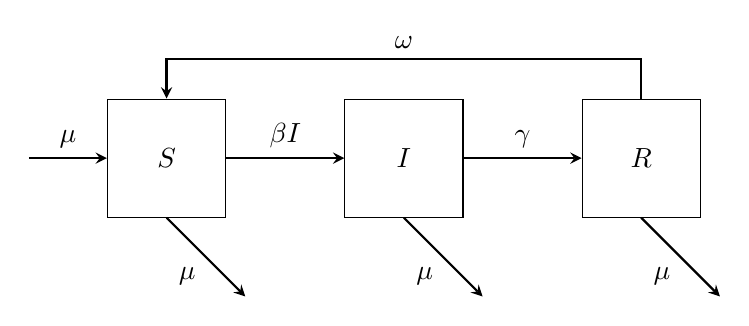
\begin{tikzpicture}[node distance=1.5cm, auto]
    \node [box](S) {$S$};
    \node [box, right=of S](I) {$I$};
    \node [box, right=of I](R) {$R$};

    \path (S.south) edge[arr] node[below left] {$\mu$} ++ (1,-1);
    \path (-1.75, 0) edge[arr] node[above] {$\mu$} (S);
    \path (I.south) edge[arr] node[below left] {$\mu$} ++ (1,-1);
    \path (R.south) edge[arr] node[below left] {$\mu$} ++ (1,-1);
    \path (S.east) edge[arr] node[above]{$\beta I$} (I);
    \path (I.east) edge[arr] node[above]{$\gamma$}(R);
    \draw[thick,->,>=stealth] (R.north) -- ++(0, .5) -| node[above,pos=.25]{$\omega$} (S.north);
\end{tikzpicture}
\caption{SIR incorporating deaths and waning immunity.}
\label{fig:sir-immunity}
\end{figure}
Note that, by sending $\omega \to 0$ we get the SIR + demography model, while sending $\omega \to +\infty$, we recover the model without immunity. The differential equations for this model are
\[
\begin{aligned}
	\dot S &= \mu - \beta IS - \mu S + \omega R\\
	\dot I &= \beta IS - (\gamma + \mu) I\\
	\dot R &= \gamma I - (\mu + \omega) R.
\end{aligned}
\]
As one might expect, the resulting oscillations are quite a bit more complex than those of the usual SIR + demography model.

\section{Session 4 (April 16)}
The main question here is about alternate parametrizations; \ie, how do we actually fit models to actually measurable data?

\subsection{Side note}

\paragraph{Flattening the curve.} ``Flattening the Curve'' is probably going to go down as the Oxford Phrase of the year of 2020. What does it mean? Essentially, thinking back to SIR model, what does this actually change?

The main reduction happens to be in $\beta$ (as one might expect). A second idea is that of interventions like HCQ or any other of the possible treatments which will do two things, either (a) hasten the recovery phase (increase $\gamma$) and also, ideally, reduce the general infectiousness as well. Sadly, none of the current treatments appear to be useful for either of these purposes and social distancing is the only thing actively working.

What's important here is that, choosing some approximate parameters for COVID-19, $\beta = 1$, $\gamma = 1/3$ (units in days), and $R_0 = 3$. Note that, even if we decrease $R_0$ by 33\%, there is only a 15\% relative reduction of the total number of cumulative cases, yet the peak amount of infections at any one point in time is substantially lowered (by around 50\%) which helps hospitals in dealing with all of this.

\paragraph{1918 Comparison.} The classic example of Philadelphia vs.\ St.\ Louis during the 1918 influenza pandemic. Philadelphia started its first case in Sep 17, holding a parade in Sep 28, and social distancing actually began in Oct 3 (far too late). The peak death rate was quite high. In comparison St.\ Louis started social distancing quite early and this led to a much smaller peak death rate (and therefore excess death rates), even though the total number of cumulative infected was approximately equal.

\subsection{Why do we need the `E' SEIR?}
We will focus on, practically, how do we actually measure the parameters? We will also chat about when we can work with SIR vs.\ SEIR.

\paragraph{SIR Assumptions.} It's rarely the case that diseases will be symptomatic immediately after infection (\ie, `incubation' periods), and SIR models total ignore these states. While mathematically convenient, the SIR model ignores this.\marginnote{A fun set of SIR models to look at and explore are those of zombie infections, which are a classic set of SIR `case' studies.}

\paragraph{Natural history vs.\ transmission intervals.} First, infections generate two periods in their natural history: first is the \emph{incubation} period, which, after symptom onset, starts the symptomatic period. In comparison to transmission intervals, where the disease has a \emph{latent} period that may or may not be infectious either before or after symptomatic onset and ending before or after. Often these are correlated, but are not necessarily equivalent.\marginnote{\emph{Incubation period:} the period before symptoms, this is distinct from the latent period or the infectious period.\\\emph{Latent period:} period before the infectious period.
\\\emph{Infectious period:} the period where someone can transmit the disease to other cases.}

For example, Whooping cough, has a latent period of 21-23 days, the infectious period is 10-11 days, yet the incubation period is 6-10 days. In contrast, measles has a latent period of 6-9 days, an infectious periods of 6-7 days, yet it has an incubation period of 8-13 days. This implies that measles has a day of potentially asymptomatic transmission, leading to difficulties in detecting it and stopping its spread.

\paragraph{How do we measure such intervals?} Almost all of the data comes from common household exposures: for example, whether people slept together, or were just present in these cases, etc. The problem with such studies is that people are consistently in contact with their household mates every day, so it's not clear when the transmission actually happened vs.\ when there was just exposure.

Another way of measuring this is to take advantage of one-off exposures at a known time. There aren't a ton of these, but SARS is one major example where these studies have appeared. The classic case is the flight from Hong Kong to Beijing and the index case was a symptomatic man 4 days into the illness, resulting in 22 people with probable secondary cases. The disease prevalence among passengers was carefully mapped and the results provided evidence against broad airborne secondary infections, but still had large amounts. Given the known day of flight and likely exposure, it was then not difficult to understand the latent period of the incubation period.

Similar studies were done for COVID-19, which showed that the median incubation period is around 5 days, with 97.5\% days developed symptoms within 9 days, and $\approx 99.9\%$ within two weeks. We are, of course, revisiting this as it seems that viral shedding continues well after symptoms are resolved.

\paragraph{On incubation periods vs.\ serial intervals.} Based on the idea that measuring the clinical onset serial interval (\ie, the interval starting after symptoms and then ending at some determined point after symptoms resolve) is easier than actually measuring the exact nature of transmission. The problem happens when, for person A, the infectious period begins well before symptoms, yet the secondary case (person B, say) has a short incubation period. This leads to negative serial intervals, which happens sometimes in the literature, but that is generally fine.

\paragraph{Emerging data on COVID-19.} A recent study looked at these periods were for COVID-19.\marginnote{See \emph{Temporal dynamics in viral shedding and transmissibility of COVID-19}.} It showed that the serial interval was around 5 days (MLE) with, of course several negative serial intervals as one might expect. The transmission distribution, with respect to the days of symptom onsets showed that transmission peaked at 1 day \emph{before} the transmission onset. And, as before, it showed the incubation period had the MLE at around 3 days. Finally, it found around 44\% of transmission in asymptomatic period.

A second study\marginnote{Spread of SARS-CoV-2 in the Icelandic Population.} found that 43\% of PCR+ confirmed cases were asymptomatic.

\subsection{(And now, finally) SEIR Models}
As one might expect, the SEIR model adds a new `exposed' state, which generates a new graph (see figure~\ref{fig:seir-deaths}).

\begin{figure}[ht!]
\centering
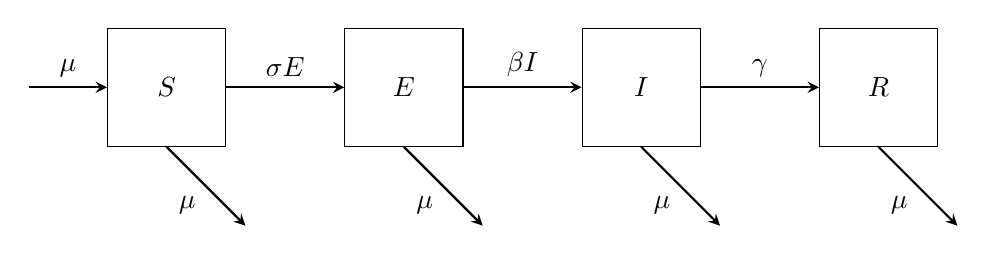
\begin{tikzpicture}[node distance=1.5cm, auto]
    \node [box](S) {$S$};
    \node [box, right=of S](E) {$E$};
    \node [box, right=of E](I) {$I$};
    \node [box, right=of I](R) {$R$};

    \path (S.south) edge[arr] node[below left] {$\mu$} ++ (1,-1);
    \path (-1.75, 0) edge[arr] node[above] {$\mu$} (S);
    \path (E.south) edge[arr] node[below left] {$\mu$} ++ (1,-1);
    \path (I.south) edge[arr] node[below left] {$\mu$} ++ (1,-1);
    \path (R.south) edge[arr] node[below left] {$\mu$} ++ (1,-1);
    \path (S.east) edge[arr] node[above]{$\sigma E$} (E);
    \path (E.east) edge[arr] node[above]{$\beta I$} (I);
    \path (I.east) edge[arr] node[above]{$\gamma$}(R);
\end{tikzpicture}
\caption{SEIR model with deaths.}
\label{fig:seir-deaths}
\end{figure}


In this case the susceptible population moves to the exposed state with a rate of $\sigma E$ (and moves to the infected with a rate of $\gamma I$). In this model. the basic reproductive number is given by,
\[
R_0 = \frac{\beta \sigma}{(\mu + \gamma)(\mu + \sigma)}.
\]
We can interpret this intuitively, by noting that, if the outgoing rates for two events are given by $r_1$ and $r_2$, then, in a uniformly sampled random interval, the probability of event 1 ocurring first is given by $r_1/(r_1 + r_2)$.

Given this, though, the duration of infectiousness ($D$) is given by $D = 1 / (\mu + \gamma)$. This means that $R_0$ in the SIR model is $\beta D = \beta / (\mu + \gamma)$, while the probability of surviving the duration of the exposed state is given by $\sigma / (\mu + \sigma)$, so multiplying these rates together, we get $R_0$ as defined above. Of course, if $\sigma \gg \mu$ (\ie, if the rate of exposure is much larger than the death rate) then we get that
\[
\frac{\sigma}{\mu + \sigma} \approx 1.
\]
(In other words, the proportion of surviving exposed is nearly one.)
\paragraph{Tuberculosis example.} While this might seem like it would be a common assumption, it turns out to not be true in TB: among those infected, only 10\% develop active TB (\ie, $p = .1$), while 90\% remain latent. An estimation is that without treatment, those with active TB infect around 10 people a year and are infectious for 2 years. This implies that
\[
R_0 = p\beta D \approx 2.
\]

\paragraph{Interventions targeting latent period.} Given someone who is exposed prophylaxis, could send them to either (a) a recovered state, or (b) a susceptible state. The problem is that in many cases we don't know which it will be. This is the idea for post-exposure therapy and is being evaluated for COVID-19 people with high-risk of exposure (and is common practice for HIV).

A question we can ask is, how effective would an intervention need to be to bring $R_0$ to less than 1? Suppose that $R_0 = 2.5$, then, assuming $p \approx 1$ without prophylaxis, we get that we would need to improve $p$ to at least $p = .4$, \ie, prophylaxis would need to reduce $p$ by at least 60\% in order to bring the new case to $R_0' < 1$.

\paragraph{Modeling growth rate more accurately.} For SARS-nCov-2, the SEIR model with $R_0 = 2.5$ latent period of 4 days, and infectious period of 5 days. The SEIR model predicts around 50 cases, while the SIR model predicts $>8000$ cases.\marginnote{This is a little clear, since infectiousness immediately after exposure would make a disease spread essentially uncontrolled.}

Surprisingly, it seems that many incubation periods typically follow log-normal distributions.

\paragraph{Distribution times in SEIR model.} Note that compartmental models actually imply that waiting times for exposure times are really \emph{exponentially distributed} which is quite different from the assumption of log-normality and can give very different results. So, this would say that most people are really in the compartments with 0.

One way of dealing with this is to add some more compartments. We can add a $n$ new compartments of latent periods, each with rates given by $n \sigma$. This is sometimes called the SE$_n$IR model. By CLT\marginnote{This is another curious thing to investigate}, we then find that the proportions then start following a log-normal distribution, which more accurately captures the known distributions.

\section{Section 5 (April 23)}
We will discuss stratification and other possible improvements to the current models, including transmission matrices.

\subsection{SIS models and stratification}
In the case of the SIS (susceptible $\to$ infected $\to$ susceptible) model, we have a single equilibrium given by
\[
\left(\frac{\beta}{\gamma}, 1 - \frac{\beta}{\gamma}\right).
\]

\paragraph{Stratified SIS.} Now, we can construct a simple stratified SIS model. Here, we generate two SIS models (with four compartments, $S_L, I_L$ and $S_H, I_H$, one for low risk and one for high) and one $\beta$ for each of the possible mixing coefficients, $\beta_{LL}$, $\beta_{LH}$, $\beta_{HL}$, $\beta_{HH}$. We will create a new matrix called the \emph{contact matrix} given by
\[
\beta = \begin{bmatrix}
	\beta_{LL} & \beta_{LH}\\
	\beta_{HL} & \beta_{HH}
\end{bmatrix}.
\]
We will say that a group is \emph{high risk} if $\beta_{HL} + \beta_{HH} > \beta_{LL} + \beta{LH}$. Additionally, we will say that the matrix is \emph{symmetric} if $\beta_{HL} = \beta_{LH}$ and the matrix is \emph{assortative} if $\beta_{HL} < \beta_{HH}$ and $\beta_{LH} < \beta_{LL}$.

\paragraph{Implications of stratification.} Obviously, if $\beta_{LH} = \beta_{HL} = 0$, then the models simply decouple and we get two individual models. On the other hand, if this is not true, it could induce interesting behavior in the two different groups where, \eg, one could see that an infection could die out in one subgroup, but then be increased again due to reintroduction from the other group.

As one might expect from the linear dynamical systems perspective, the general dynamics will follow those of the group with the largest eigenvalue of $\beta$. Additionally, stratified models can sustain an endemic equilibrium with relatively low \emph{overall} prevalence (though there is a higher fraction of the $H$ subgroup that is infected).


\paragraph{Control measures.} We can add a new compartment to the SIS model, a vaccinated compartment $V$, which removes those from the susceptible pool (and places them into the new pool $V$) at some specific rate. The question is, how many people do we need to vaccinate for optimal control? And how targeted should the vaccinations be? (How many from each of the $H$ and $L$ subgroups are needed?)\marginnote{This could lead to an interesting control problem over time, especially with uncertainty; the result could lead to an MDP, for example.}

\paragraph{Inference.} How do we infer the matrix $\beta$? If we assume that contacts occur at random between people of types $i$ and $j$, and the fraction of contacts is (XXX complete, not clear from slides)

In this partnership model, we can then directly derive $R_0$ from the mean $M$ and variance $v$ of the number of partners (XXX: check this)
\[
R_0 = \frac{\beta}{\gamma}\frac{M^2 + V}{V}.
\]
Note that this random partnership model is not assortative. We can add an additional term $\alpha$ which displays an additional preference of people of a given group to mix with those of the same group. To do this, take a convex combination (with weights $\alpha$ and $1-\alpha$) of this model and the perfectly isolated model.\marginnote{How about a convex problem? This is a question of inferring essentially a PSD matrix.}

\paragraph{Survey methods.} Another approach to establish empirical mixing patterns, we can also easily survey people about their behaviors/contacts. This is simple in the case of, say STDs, but hard when you consider respiratory diseases. You can also construct a transmission graph by simply asking how many people each person had, and then attempt to reconstruct the corresponding graph from it, which can then be used to build its mixing matrix, where each row and column represents a compartment, which is stratified by the number of people who someone has had relationships with.

\subsection{Risk stratified models}
Recall that the SIR model with demographics has a damped oscillatory equilibrium (in the endemic case). In this model, people stayed in their age groups.

Note that people move from one age to another age group in a fairly predictable manner. This creates flows between the susceptible, infected, and recovered compartments of each of the models (which is independent of the infections and coefficient matrix between them!). What are the resulting dynamics?

\subsection{Fixed and time varying parameters}
A simple example of this is to have a time-varying contact parameter. One specific case is to have a simple oscillatory contact parameter:
\[
\beta = \beta_0(1 + \cos(\omega t)),
\]
for some oscillation $\omega$. Now, if $\omega$ is close to the equilibrium oscillation period, you get fun resonances (\eg, forcing) which yields some specific spiking behavior.




\end{document}

